\chapter{Aspectos básicos de la inversión bursátil}

\section{Objetivos}

\begin{itemize}
    \item Saber diferenciar entre \ti{operativa a largo plazo} y \ti{operativa a corto plazo}.
    \item Entender que, en el largo plazo, la inversión en bolsa es la mejor opción.
    \item Saber qué efecto puede tener la diversificación en mis inversiones.
    \item Conocer el papel que juegan los dividendos en mis decisiones de inversión.
\end{itemize}

\section{Primeros pasos}

¿Cuál es nuestro objetivo?. Rentabilizar capital, ganando dinero de forma consistente y con un riesgo limitado.

Opciones de activos financieros en los que invertir:
\begin{itemize}
    \item Destinar nuestro capital a un \ti{depósito bancario}. La rentabilidad es muy baja.
    \item Invertir en \ti{renta fija}, es segura y con un riesgo mínimo, su rentabilidad también es bastante baja.
    \item Invertir en \ti{renta variable}, más favorable que las anteriores, nos permite invertir en
    \begin{itemize}
        \item acciones
        \item en CFD's
        \item futuros, \ldots
    \end{itemize}
    \item En \ti{fondos de inversión}, que pueden combinar alguno de los activos que hemos visto.
\end{itemize}

Las dos últimas suelen ser preferibles a las primeras, sobre todo a largo plazo ya que nos darán mayor rentabilidad.

¿Qué tipo de inversor podemos ser?. Básicamente tenemos dos tipos:
\begin{itemize}
    \item \tb{Inversor a largo plazo}, personas que tienene un capital determinado en la actualidad o que prevén que van a ir acumulando a lo largo de los años, lo que que quiere es rentabilizar ese capital. En este caso, el mejor consejo sería realizar una \tb{gestión pasiva}, es decir, alguien que no tiene tiempo para dedicarse a seguir la bolsa diariamente o que tenga como fuente de ingresos otra actividad que no es la de inversor.
    \item \tb{Inversor a corto plazo},  son aquellas personas cuya principal fuente de ingresos la \ti{especulación bursátil} (también denominado especulador o trader), tiene que seguir una \ti{gestión activa}, estar pendiente de la evolución de las cotizaciones, de la revalorización de los diferentes activos financieros; tiene que saber cuando entrar y cuando salir en el mercado con qué cantidad, etc.
\end{itemize}

Nos centramos en las premisas del primer tipo de inversor, \ti{a largo plazo}:

\begin{enumerate}[label=\alph*)]
    \item Su objetivo es rentabilizar el capital. Cubrirse de la \ti{inflación} de forma que su capital al menos mantenga su poder adquisitivo. Introducimos dos conceptos que son:
    \begin{itemize}
        \item \tb{interés simple}
        \item \tb{interés compuesto}
    \end{itemize}


    \begin{testexample}[ Pongamos que queremos adquirir un vehículo, y que ese vehículo en la actualidad, tiene un coste de 10000€, ese sería su precio. Supongamos que la inflación crece a un ritmo de 2\% anual, es decir, el precio de los activos, incluido el de este vehículo, va a subir anualmente de manera acumulada un 2\%. ¿Cómo evolucionará, en 10 años. el coste del vehículo?]
        \begin{equation*}
            \begin{split}
                t &= 0 \rightarrow \euros{10.000} \\
                t &= 1 \rightarrow  (10.000 + 2\%) x 10.000 = 10.000 x (1 + 2\%) = \euros{10.200} \\
                t &= 2 \rightarrow (10.200 + 2\%) x 10.200 = 10.200 x (1+2\%) = 10.000 x (1+2\%)^2 = \euros{10.404} \\
                t &= 10 \rightarrow (10.000 x 1+2\%)^{10} = \euros{12.189,94}
            \end{split}
        \end{equation*}

        Hemos empleado la \ti{ley de interés compuesto} frente al \ti{interés simple}, puesto que lo que hacemos es que los incrementos se acumulan sobre los valores anteriores, es decir, el incremento en el precio del vehículo no es \ti{200€} al año, sino que es del 2\% siempre sobre el último valor considerado, que hemos calculado. De haber utilizado el \ti{interés simple} el resultado habría sido de \euros{10.400}.

        Podríamos hacernos la pregunta de ¿cuál será el poder adquisitivo de \euros{10.000} actuales dentro de 10 años?.
        \begin{equation*}
            \begin{split}
                t &= 0 \rightarrow \euros{10.000} \\
                t &= 1 \rightarrow \frac{10.000}{(1+2\%)} = \euros{9.803,92} \\
                t &= 3 \rightarrow \frac{9.803,92}{(1+2\%)} = \frac{10.000}{(1+2\%)^2} = \euros{9.611,68} \\
                t &= 10 \rightarrow \frac{10.000}{(1+2\%)^{10}} = \euros{8.203,48}
            \end{split}
        \end{equation*}
    \end{testexample}

    La inversión bursátil lo que nos permite es defendernos de la pérdida de poder adquisitivo dada por el efecto de la inflación.

    Si nuestro dinero no se invierte, perderemos poder adquisitivo por dos vías:
    \begin{itemize}
        \item por el efecto de la inflación.
        \item por el coste de oportunidad, no haberlo rentabilizado a través de una inversión.
    \end{itemize}

    Con el siguiente ejemplo podemos analizar el efecto de estas dos situaciones.

    \begin{testexample}[ Imaginemos disponer de \euros{50.000} que podemos invertir durante los próximos 20 años al 5\% anual.]
        \begin{itemize}
            \item Si no lo invertimos, la tasa de la inflación sigue siendo del 2\% anual, el poder adquisitivo dentro de 20 años de los \euros{50.000} se reduzca hasta \euros{33.648.57}.
            \item Si los invierto al 5\%, y teniendo en cuenta la inflación, el poder adquisitivo alcanzará los \euros{89.279.66}
        \end{itemize}
    \end{testexample}
    
    \item Mejor opción, la \tb{renta variable}, invirtiendo que no se necesite, ni ahora ni en el corto/medio plazo.
    \item Diversificar.
    \item Reinvertir dividendos, siempre que se invierte en acciones, por el principio de que la bolsa en largo plazo es siempre alcista; reinvirtiendo los dividendos nos vamos a asegurar:
    \begin{itemize}
        \item una mayor rentabilidad
        \item una serie de ventajas fiscales.
    \end{itemize}
\end{enumerate}

\section{Renta variable en el largo plazo}

En la renta variable siempre se obtiene rentabilidad por dos vías:
\begin{enumerate}
    \item por las plusvalías, mayor valore de los activos a medida que pasa el tiempo, por la revalorización de sus activos.
    \item por los dividendos que dan las empresas, en el caso del IBEX35 de acuerdo con la serie histórica está entorno al 5\%.
\end{enumerate}

Si observamos las gráficas correspondientes al índice IBEX35 y a la seríe histórica del Down-Jones podemos ver que la inversión a largo plazo siempre es alcista.

Tenemos dos formas de presentar los gráficos:
\begin{itemize}
    \item mediante la \ti{escala aritmética}
    
    \begin{center}
        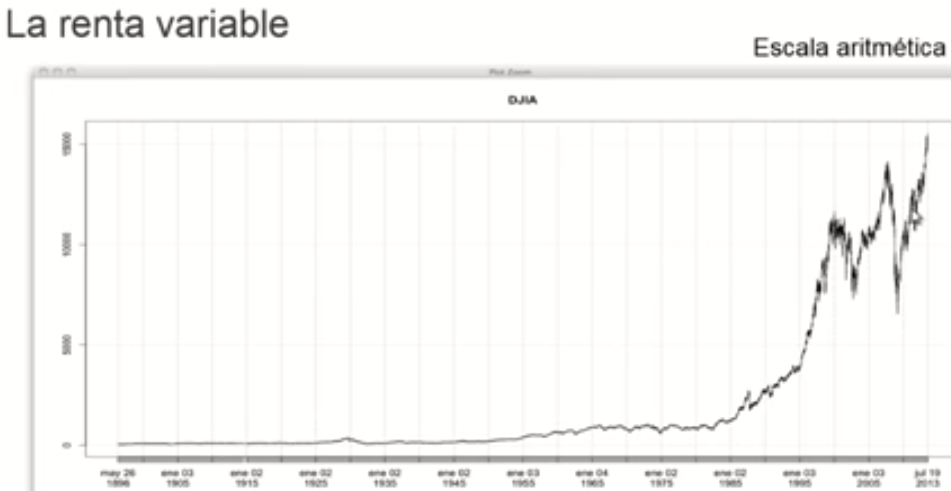
\includegraphics[scale=0.35]{images/rv-aritmetica.png}    
    \end{center}
    
    \item mediante la \ti{escala geométrica}
    
    \begin{center}
        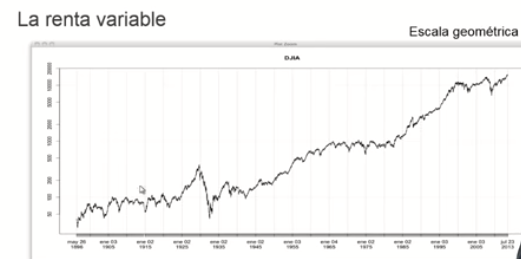
\includegraphics[scale=0.75]{images/rv-geometrica.png}    
    \end{center}
    
    En esta escala, básicamente cambiamos el eje de las \ti{y}, vemos que el paso de 50 a 100 puntos supone un incremento del 100\%, esa diferencia es la misma para pasar de 100 a 200 puntos, el incremento es del 100\%. Es decir, representamos con la misma escala los incrementos porcentuales, no los incrementos absolutos. En esta gráfica estamos representando los mismos valores desde el año 1896 a la actualidad del Down Jones. Ahora, comparando ambas gráficas podemos ver, con mayor claridad, la pérdida porcentual que supuso las crisis del 29, y podemos ver que en esta serie histórica, la crisis más importante fue la del año 29, que quedaba oculta en la escala artimética, así como las correspondientes a 2000 y 2008, aún siendo importantes, se aprecia que no fueron tan fuertes. Esta \ti{escala logarítmica} nos permite ver la clara tendencia alcista de la bolsa en el largo plazo y, por lo tanto, sería una posibilidad de inversión, no para los que quieran rentabilidad el capital en dos o tres años, sino para los que quieran construir su propio plan de pensiones o fondo de inversión invirtiendo en \ti{renta variable}, en \ti{acciones}.
\end{itemize}


\section{Diversificación}

Estamos en la suposición del \ti{inversor a largo plazo}.

La \tb{diversificación} es un concepto introducido por el \ti{Premio Nobel de Economía de 1990 Harry Markowitz}, por sus trabajos sobre \ti{«Selección de carteras eficientes de carteras óptimas»}; su principal aportación al campo de las finanzas fue que cualquier decisión bursátil debe considerar dos parámetros:
\begin{itemize}
    \item la rentabilidad.
    \item el riesgo.
\end{itemize}
que, además, están contrapuestos entre sí, aquellos activos que nos pueden ofrecer mayor rentabilidad en el largo plazo, por lo general, también van a ser los que más riesgos tengan, mientras que los que tengan una rentabilidad menor en el largo plazo, también serán los más seguros en el largo plazo, con menor riesgo.

Lo que no debemos hacer, y es un error típico de todo el que se acerca por primera vez al mundo bursátil, es invertir todo nuestro capital, el destinado a invertir, en un único activo, por lo tanto, \ti{debemos diversificar nuestra inversión entre diferentes activos}, si podemos nos interesa diversificar en diferentes sectores productivos e incluso en diferentes países. Cuanto más diversificado esté nuestro portfolio, cartera de inversión, de forma más eficiente trataremos el riesgo sin reducir nuestra rentabilidad en el largo plazo.

Tampoco es conveniente invertir en acciones de empresas que sean muy pequeñas con un accionariado muy concentrado donde las acciones están concetradas, en mayor cuantía, en un número reducido de inversores, porque éstos pueden \ti{"alterar la cotización del título"}, comprando o vendiendo grandes paquetes, haciendo que la cotización suba o baje a su antojo, lo que puede repercutir en los pequeños accionistas.

El concepto de \tb{riesgo} está asociado a la \ti{volatilidad de las cotizaciones}, como muestra el gráfico:
\begin{center}
    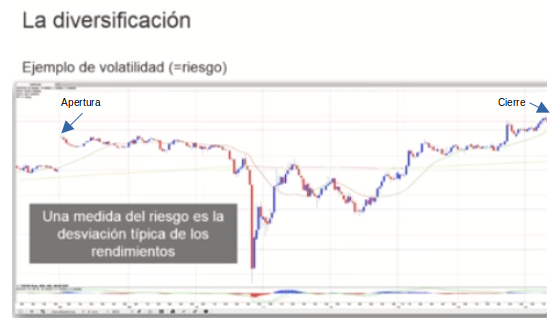
\includegraphics[scale=.75]{images/diversificacion-riesgo.png}
\end{center}
Tenemos representada la cotización en el índice alemán DAX a lo largo de un día concreto. En la evolución intra-día de ese índice, el precio parte, en la parte izquierda el gráfico, con un ligero \ti{gap} respecto del día anterior y a lo largo de la mañana se producen ligeros movimientos de alza y baja, que oscilan, pero llegado un momento concreto rompe con fuerza hacia abajo y luego, casí inmediato, recupera el valor anterior, incluso al final del día acabar con un precio de cierre superior al de apertura, es decir \ti{rentabilidad positiva}.

Observamos fluctuaciones muy fuertes en el precio de la cotización, esto es la volatilidad, el riesgo, es lo que no nos interesa a largo plazo, y por qué no nos interesa aunque finalmente se acabe ganando dinero, si uno h comprado el índice, va haber momentos en los cuales vamos a ir prediendo una cantidad muy importante de dinero y en el momento de recuperarse vender, no obteniendo los rendimientos finales. También observamos que hay diferentes puntos a lo largo del día donde podríamos comprar, pero están igualmente sujetos a momentos de caídas y pérdida y posterior recuperación.

Uno nunca sabe realmente el momento idóneo para realizar una entrada en un activo, por lo tanto, lo que nos interesa es que haya las menores fluctuaciones posibles, lo que hace que a lo largo de vida de la inversión soportaremos pérdidas pequeñas, que finalmente se acaban recuperando. Veamos un par de casos qeu clarifiquen lo visto y tener claro en qué consiste el \ti{concepto de diversificación}.

\begin{itemize}
    \item Decidimos invertir en un único activo. Podemos llevarnos sorpresas positivas, como es el siguiente caso en el que vemos la cotización de la empresa \ti{Jazztel}:
    \begin{center}
        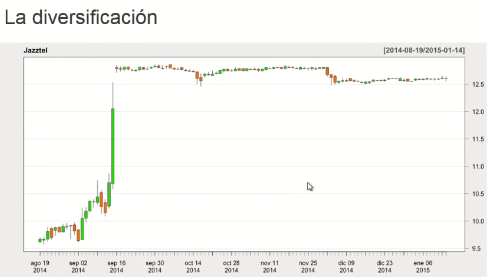
\includegraphics[scale=0.65]{images/jazztel.png}
    \end{center}
    Quienes compraron en torno a los 10€ vemos como prácticamente en una semana obtuvieron una rentabilidad del 25\% de su inversión.
    \item Este otro gráfico se refiere a otra empresa español \ti{FCC}:
    \begin{center}
        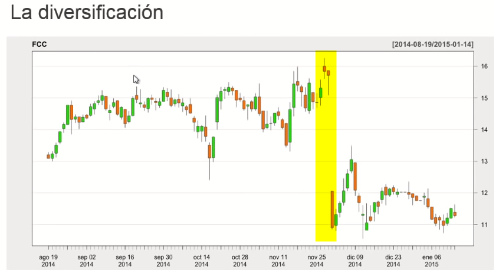
\includegraphics[scale=0.65]{images/fcc.png}
    \end{center}
    Los que decidieron comprar en la parte superior de la zona amarilla, se encontraron, en un único día, una bajada en torno al 30\%, perdieron un 30\% de lo invertido. 
\end{itemize}

Esto quiere decir que si invertimos el 100\% de nuestro capital en un único activo puede que nos vaya bien, caso 1, o muy mal como en el segundo caso. Por eso es recomendable no invertir en un único título (activo), sino diversificar.

Cómo podemos diversificar, a través de un \ti{\tb{índice bursátil}}, por ejemplo en el \ti{IBEX-35}, que se compone de los treinta y cinco títulos de mayor capitalización bursátil del mercado español.
\begin{center}
    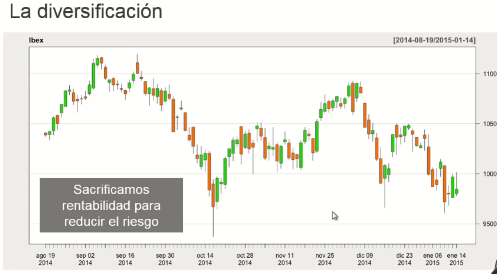
\includegraphics[scale=0.65]{images/diversificacion-ibex35.png}
\end{center}
Para este período, de prácticamente seis meses, la cotización se ha movido entre los once mil puntos y llegado a bajar hasta los nueve mil quinientos, observamos una fluctuación del 10\% y el 15\%. En el caso de FCC vimos que en un sólo día llego a perder el 33\% de la inversión, del gráfico vemos que diversificar reduce esta volatilidad.

La inversión en un índice bursátil no tiene por qué restringirse a un índice de un país, podríamos diversificar entre índices de diferentes países. Existen diferentes mecanismos:
\begin{itemize}
    \item \tb{Fondo de Inversión}, están sujetos a comisiones de mantenimiento, etc, que suelen ser bastante elevadas.
    \item Invertir en un \tb{ETF}, que también replica el comportamiento del índice bursátil, también hay comisiones, que a priori pueden parecer pequeñas, pero conforme se acumulan en el tiempo acaban siendo importantes, mermando nuestra rentabilidad final.
    \item Otra forma es que uno mismo seleccione los títulos que van a formar parte de nuestra cartera. Tengo 35 títulos a disposición, este año puedo invertir en tres de ellos, el año siguiente elijo otros o amplio, de forma que formo mi propia cartera cada año, finalmente obtendré un recorrido muy similar al que podría obtener el IBEX-35.
\end{itemize}

\section{El papel de los dividendos}

Lo que vamos a ver es como afecta la \ti{re-inversión de dividendos} a la rentabilidad de nuestra cartera de inversión en el largo plazo.

Veremos dos importantes conclusiones:

\begin{itemize}
    \item Obtendremos un importante revalorización de nuestra inversión, de nuestra rentabilidad.
    \item Conlleva una serie de ventajas fiscales que inciden positivamente en la rentabilidad de nuestra inversión.
\end{itemize}

Veamos un sencillo ejemplo y luego lo veremos en la práctica real.

\begin{center}
    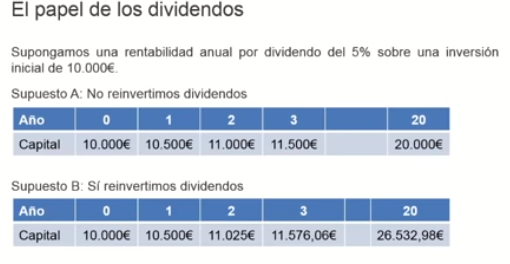
\includegraphics[scale=.90]{images/papel-dividendos.png}
\end{center}

Vamos a suponer que obtenemos una rentabilidad anual por dividendo del 5\% sobre una inversión inicial de \euros{10.000}. Planteamos dos supuestos:
\begin{enumerate}
    \item No invertiremos los dividendos de ese 5\%; el capital inicial será de \euros{10.000}, obteniendo un 5\% el capital dentro de un año  será de \euros{10.500}, el tercer año \euros{11.500}, en el largo plazo, en veinte años se habrá convertido en \euros{20.000}, es decir, una rentabilidad por dividendo del 5\% nos asegura doblar el capital en un período de 20 años, un incremento del 100\%.
    \item Re-invertimos los dividendos del 5\%, lo destinamos a la compra de nuevas acciones. Inicialmente partimos del mismo capital del caso anterior, \euros{10.000}, pero en lugar no re-invertir los dividendos obtenidos, los \euros{500} obtenidos sirven para comprar acciones, la rentabilidad para el año 2 no se establece sobre el capital inicial, sino sobre los \euros{10.500} que teníamos al final del año 1, obtendrías \euros{11.025}, la diferencia respecto al caso anterior es muy pequeña, sólo \euros{25}. Para el año 3 obtenemos \euros{11.576,06}, son \euros{76,06}, la diferencia relativa en términos porcentuales entre una y otra opción es muy pequeña. ¿Qué ocurre en el largo plazo?. vemos que al cabo de 20 años, los \euros{10.000} se convirtieron en \euros{26.532,98}, hemos obtenido más de \euros{6.500} respecto de la primera opción, hemos conseguido un incremento del 160\%.
\end{enumerate}

No sólo obtendremos una rentabilidad mayor, ya que partimos de la inversión a largo plazo es alcista, sino que también tendremos una mayor rentabilidad debida al efecto fiscal de los dividendos.

Supongamos que nos retienen un 21\% de los dividendos que obtenemos, significa que si no se re-invierten los dividendos, ese 5\% de \euros{500}, tendremos que pagar al fisco el 21\%, lo que nos queda neto son \euros{395} y no los \euros{500}.

\begin{center}
    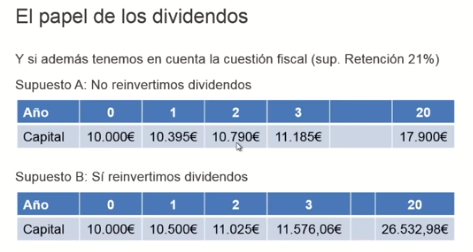
\includegraphics[scale=.90]{images/papel-dividendos-fiscal.png}
\end{center}

Para el segundo año obtendríamos \euros{10.790}, de nuevo el fisco se queda con un 21\% del 5\% obtenido por dividendos, y así sucesivamente. A los 20 años obtendríamos \euros{17.900}. Es decir, al no re-invertir, el fisco obtuvo un 21\% cada año del 5\% de nuestros beneficios, ya no tendríamos una rentabilidad del 100\%, hay que restarle el 21\% y nos queda una rentabilidad del 69\%.

Por el contrario, si reinvertimos los dividendos, en lugar de recibir los dividendos en \ti{líquido} lo recibo en \ti{acciones}, no me retendrán el 21\%, ya que no estoy recibiendo el dividendo en euros, por lo tanto, no hay retención. En este caso los \euros{10.000} acabarán convirtiéndose en \euros{26.500}, haciéndose más notable la diferencia entre ambas opciones.

¿Qué rentabilidad esperemos tener por nuestra inversión bursátil vía dividendos?.¿Cuál es ls rentabilidad media histórica que ofrecen las empresas vía dividendos?.

\begin{center}
    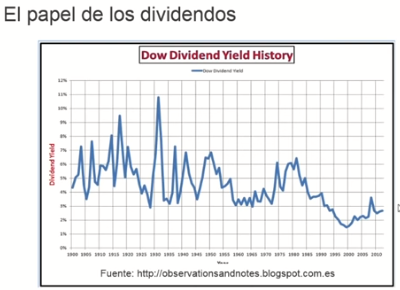
\includegraphics[scale=.70]{images/dividendos-historico.png}
\end{center}
El gráfico muestra el \ti{histórico de rentabilidad por dividendos del índice americano Dow Jones}, donde un períod de tiempo desde el inicio hasta la década de los 90, el índice ha estado, normalmente, por encima del 3\%, llegando en ocasiones a superar el 10\%, la media ha estado entre el 3\% y el 5\%. Ahora estamos en un período históricamente bajo, con rentabilidades entre el 2\% y el 3\%, en otros países, como el caso español, es algo mayor en torno al 5\%.

La siguiente gráfica es muy interesante, un trabajo de un investigador americano que parte del siguiente supuesto: imaginemos que hubiéramos realizado nuestra inversión justo al inicio de la crisis bursátil de 1921. ¿Qué hubiera ocurrido si nuestra inversión no hubiera tendio en cuenta los dividendos? y ¿qué hubiera ocurrido si tenemos en cuenta la rentabilidad adicional que nos proporcionan los dividendos?.
\begin{center}
    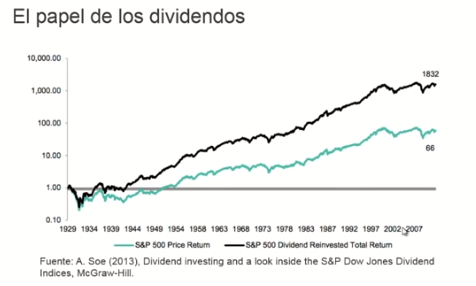
\includegraphics[scale=.80]{images/papel-dividendos2.png}
\end{center}
Pues si hubiéramos invertido en la \ti{S\&P500} en este año, un dólar se habría convertido ha finales de 2007 y principios de 2008 en 66\$, es decir, habríamos multiplicado por sesenta y seis el capital inicial, sin tener en cuenta los dividendos. La rentabilidad que habríamos tenido, si los tenemos en cuenta, ese dólar se habría convertido en \ti{1.832\$}, por lo tanto, es \ti{muy importante, en el largo plazo, considerar la rentabilidad vía dividendos} porque la diferencia son muy significativas.

En la gráfica vemos lo que ocurre con un período de tiempo muy largo, pero luego lo que veremos, en los ejercicios, es cuál es el efecto de los dividendos para una rentabilidad media de 15 o 25 años. Veremos también que las diferencias son muy significativas.

Como cuestiones a tener en cuenta:
\begin{enumerate}
    \item invertir en dividendos supone recibir acciones en lugar de recibir efectivo.
    \item ¿Tenemos que invertir sólo en acciones con alta rentabilidad por dividendo, sólo acciones españolas, americanas, alemanas, \ldots?. La respuesta es \tb{no}, el precio de la acción ya descuenta todo, entre otras cosas el dividendo. La cotización de la acción justamente bajará el 5\% porque es dinereo que sale del patrimonio de la empresa, por lo tanto, la empresa es menor y eso incide en la cotización del activo. 
    Por lo tanto, no necesariamente hemos de invertir en empresas que nos den una alta rentabilidad por dividendo, aquí también es importante diversificar y conjugar empresas que dan una rentabilidad limitada por dividendo como aquellas que nos aseguren una rentabilidad importante sostenida en el largo plazo.
\end{enumerate}
